\documentclass[12pt, a4paper,usenames,dvipsnames]{article}
\usepackage[utf8]{inputenc}
\usepackage[english]{babel}
\usepackage{amsmath,amssymb,amsthm} 
\usepackage{graphicx}
\usepackage{siunitx}
    \sisetup{exponent-product = \cdot} 
    \sisetup{separate-uncertainty = true}
\usepackage[margin=20mm, tmargin=30mm,headheight=15pt ]{geometry}
\usepackage{fancyhdr}
\usepackage{framed}
\usepackage{caption}
\usepackage{subcaption}
\usepackage{lastpage}  
\pagestyle{fancy}
    \fancyhf{}
    \rhead{Project 3}
    \lhead{MA2501}
    \rfoot{Page \thepage \ of \pageref{LastPage}}
\fancypagestyle{noheader}{
  \fancyhf{}% Clear header/footer
  \renewcommand{\headrulewidth}{0pt}% No header rule
  \rfoot{Page \thepage \ of \pageref{LastPage}}
}
\usepackage{tikz}
\usetikzlibrary{calc}
\usetikzlibrary{patterns}
\usetikzlibrary{positioning}
\usepackage{lettrine}
\title{Project 3 - MA2501}
\author{Anna Bakkebø\And Thomas Schjem \And Endre Sørmo Rundsveen}
\usepackage{sectsty}
\usepackage{bm}


\definecolor{XKCDpale}{RGB}{255,249,208}
\definecolor{XKCDcrimson}{RGB}{140,0,15}
\definecolor{XKCDpalegray}{RGB}{253,253,254}

\sectionfont{\color{XKCDcrimson}}
\subsectionfont{\color{XKCDcrimson}}
\usepackage{listings}%Code show
\lstdefinestyle{mystyle}{
    backgroundcolor=\color{XKCDpalegray},
    commentstyle=\color{YellowGreen},
    keywordstyle=\color{XKCDcrimson}\bfseries,
    numberstyle=\tiny,
    stringstyle=\color{OliveGreen},
    basicstyle=\footnotesize,
    breakatwhitespace=false,         
    breaklines=true,                 
    captionpos=t,                    
    keepspaces=true,                 
    numbers=left,                    
    numbersep=1pt,                  
    showspaces=false,                
    showstringspaces=false,
    showtabs=false,                  
    tabsize=1,
    xleftmargin=0.5em,
    frame=topline
}
 
\lstset{style=mystyle}
\renewcommand\vec{\mathbf}

\begin{document}

\begin{titlepage}
    \newgeometry{margin=20mm,tmargin=110mm}
    \begin{tikzpicture}[remember picture,overlay]
        \fill[color=XKCDpale] ($(current page.south west)+(0cm,15cm)$) rectangle (current page.north east);
        \foreach \x in {2,3,4,5,6,7,8}
            {\fill[gray!40] (\x cm, 1)--(\x cm, {3+1.15*sin(0.5*pi*\x r)*exp(-\x/4)})--(\x +1,{3+1.15*sin(0.5*pi*(\x+1) r)*exp(-(\x+1)/4)})--(\x +1,1) --cycle;
            \draw[dashed] (\x cm, {3+1.15*sin(0.5*pi*\x r)*exp(-\x/4)})--(\x +1,{3+1.15*sin(0.5*pi*(\x+1) r)*exp(-(\x+1)/4)});}
        \draw[thick,->] (-2,1)--(15,1);
        \draw[thick,->] (-2,1)--(-2,8);
        \foreach \x in {2,3,4,5,6,7,8,9}
            {\draw (\x cm,1cm+2pt)--+(0,-4pt);
            \draw[dashed] (\x ,1)--(\x,{3+1.15*sin(0.5*pi*\x r)*exp(-\x/4)});}
        \node[anchor=north] at (2,1){\(a\)};
        \node[anchor=north] at(9,1){\(b\)};
        \draw[Mahogany, thick, domain=2:9] plot[samples=100] (\x, {3+1.15*sin(0.5*pi*\x r)*exp(-\x/4)});
        
    \end{tikzpicture}
  
    {\noindent \Huge \color{Brown}{\underline{Project 3 - MA2501}}}\\
    
    {\noindent\large \color{Brown}{Anna Bakkebø\\Thomas Schjem\\Endre Sørmo Rundsveen}}\\
    \raggedright
    \hfill \break
    \lettrine[lraise=0.15]{T}{} his document is the report for our third project in Numerical Methods - MA2501 the spring semester of 2019. The project mainly focuses on numerical integrations techniques and are based on the Newton-Cotes quadrature formula. First we familiarize ourself with the adaptive simpson method, before we continue with the Romber method, and lastly we end by exploring both the Runge-Kutta implicit integration method and the improved Euler method. 
    % \begin{lstlisting}[language=Python]
    % import matplotlib
    % import matplotlib.pyplot as plt
    % import numpy as np
    % import sumpy as symp\end{lstlisting}
\end{titlepage}
\restoregeometry
\twocolumn

\section*{Problem 1}
\subsection*{a)}
The composite Simpson method is a method which takes the interval given and 
\subsection*{c)}
\newpage
gbbr
\newpage
\thispagestyle{noheader}
\onecolumn
\newgeometry{margin=20mm, tmargin=0.61\paperwidth,headheight=15pt}
\refstepcounter{figure}
\label{fig:graph}
\begin{tikzpicture}[remember picture,overlay]
    \fill[color=XKCDpale] ($(current page.north west)-(0,{0.6\paperwidth})$) rectangle (current page.north east);
    \node (graph) at ($(current page.north)-(0,0.3\paperwidth)$) {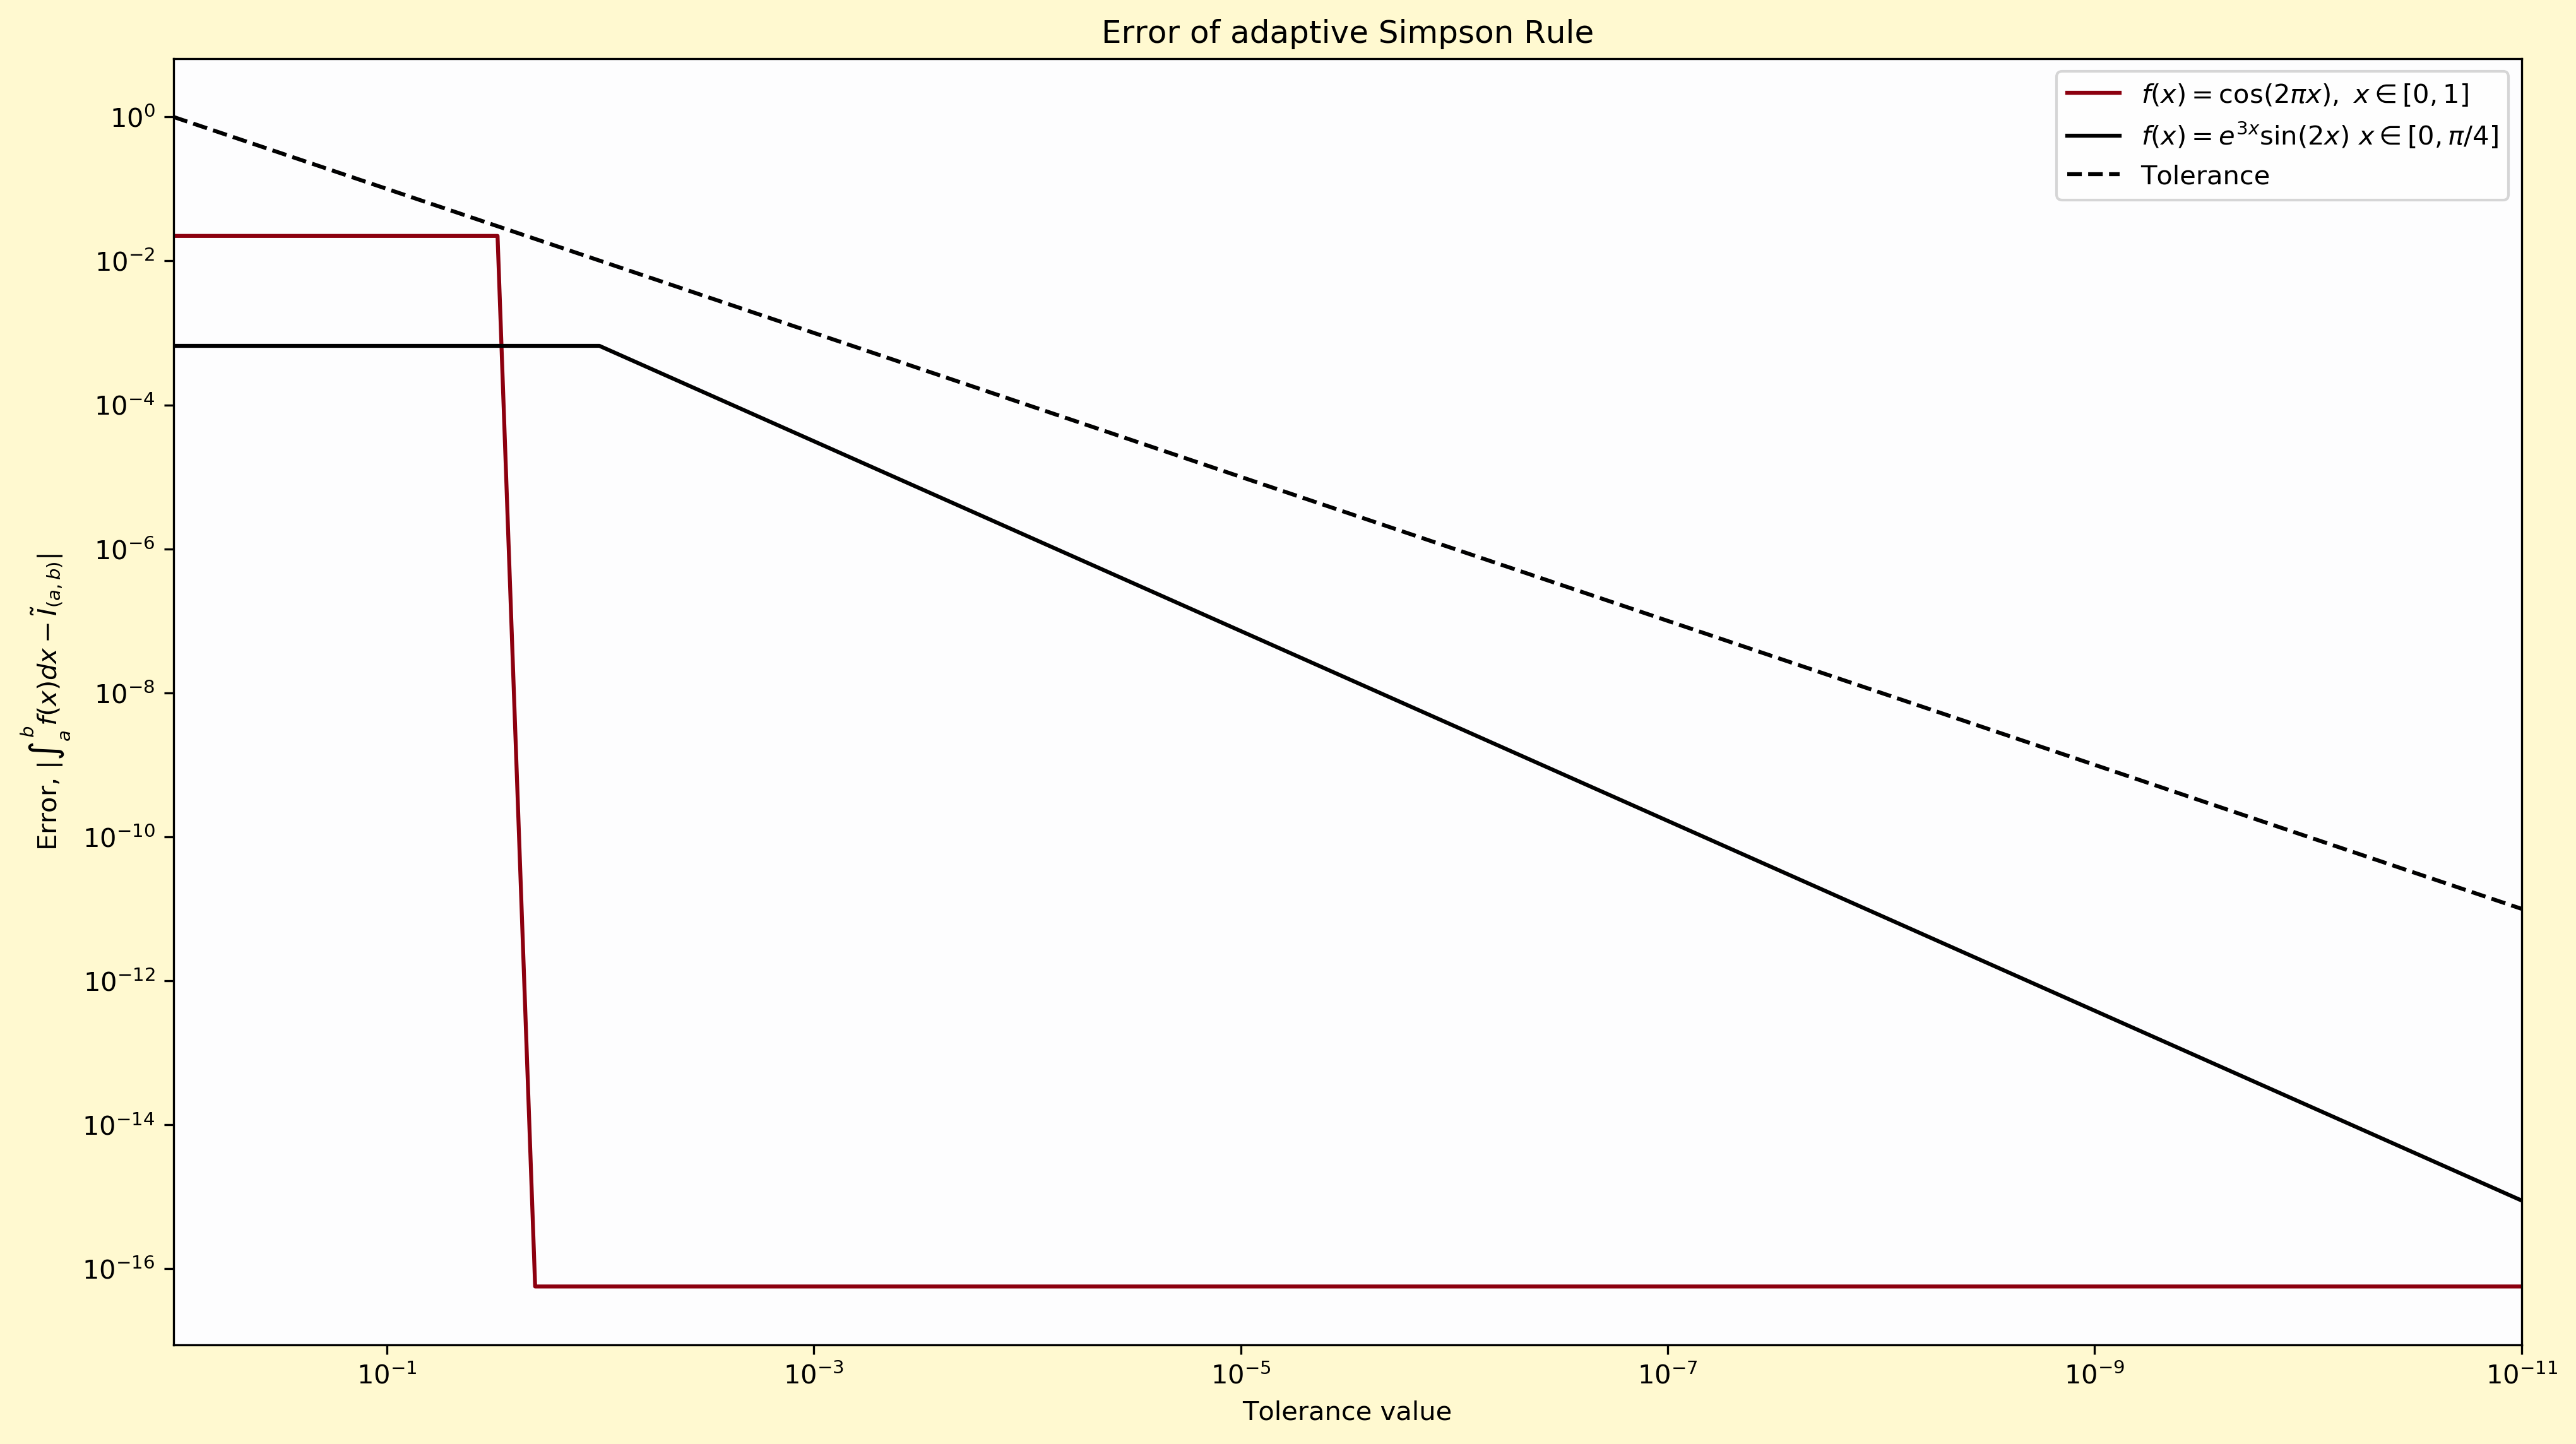
\includegraphics[width=0.9\paperwidth]{pltAdpSimp.png}};
    \node[below= 0.15cm  of graph] {Figure \arabic{figure}: The errors of the adaptive Simpson Rule with decreasing tolerance, for different functions.};
\end{tikzpicture}

\restoregeometry

\end{document}
